\chapter{Development phases}
\label{chapter3}

In this chapter, we introduce the division and scheduling of every process that needs to be carried out in order to complete the project that is presented in this DFP. A Gantt chart is provided describing the actual time allocated to each of the tasks, as well as some additional graphs and charts presenting other details of the followed schedule.

\section{Gantt chart}

Since the original planning, the total work to be done had been organized into the \textit{6 development phases}, each of them as well divided into a set of subprocesses, that are detailed in the Gantt chart in Figure \ref{fig:gantt}.

\begin{figure}[h]
  \centering
  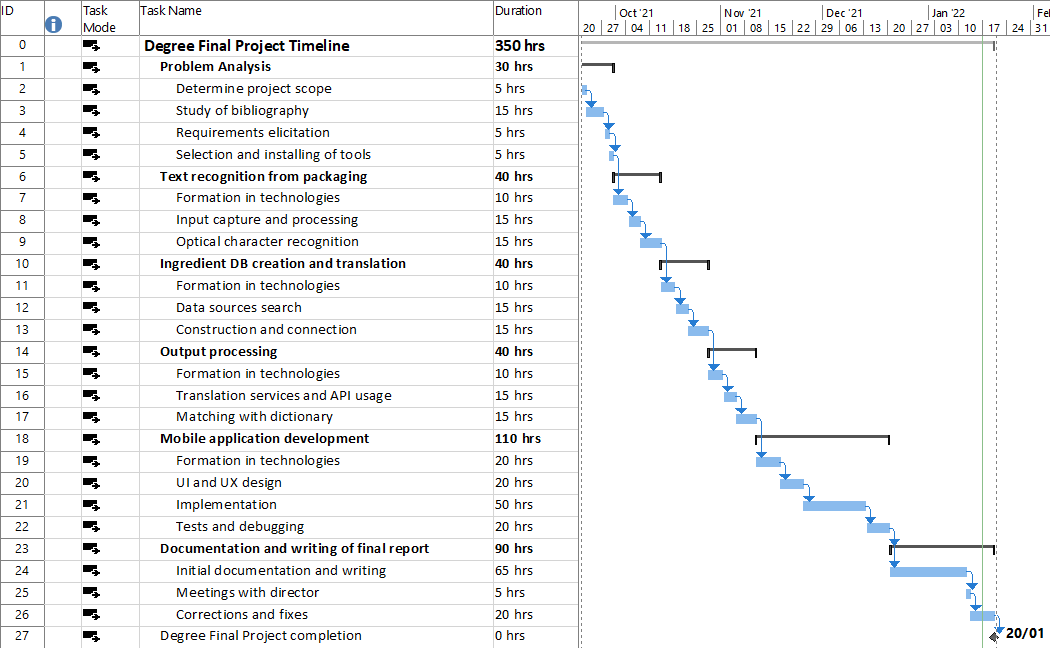
\includegraphics[width=\textwidth]{Figures/gantt.png}
  \caption{%
    Gantt chart for the development of the DFP
  }
  \label{fig:gantt}
\end{figure}

The timing had originally been estimated for work days of 20 hours per week, adding to a total of \textit{300 hours} of work over \textit{15 weeks}. While this calculation was made according to the DFP guidelines, it ended up underestimating the actual time that some of the processes took to complete, such as the time designated to the implementation and coding of the app or to the writing of this document. With these adjustments, the total time dedicated was approximately \textit{350 hours} of work, executed over \textit{17.5 weeks} or roughly 4 months.

An extended version of this Gantt chart (Figure \ref{fig:gantt_actual}), as well as the Gantt chart used in the original planning (Figure \ref{fig:gantt_planned}) for comparison reference, are available on appendix \ref{appendix:A}.

\subsection{Timeline}

In Figure \ref{fig:timeline}, we can see the timeline view of the project with the start and ending dates for each of the milestones. As the development followed a sequential approach, there was no overlapping between any of the processes and each of them was started only as the previous one finished. The initial four tasks spanned over the first two months of development, while another two months were dedicated to the two final tasks.

\begin{figure}[h]
  \centering
  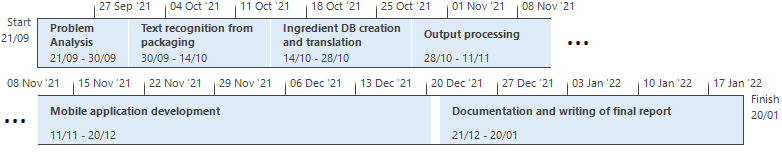
\includegraphics[width=\textwidth]{Figures/timeline.png}
  \caption{%
    Timeline for the development of the DFP
  }
  \label{fig:timeline}
\end{figure}

\section{Time distribution}

As shown in Figure \ref{fig:ganttbars}, the time distribution across all of the 6 processes was quite uneven, with some of the tasks demanding almost twice as much time as others. In particular, the coding and implementation of the app, as well as the writing of this report, took more time than all of the remaining tasks combined.

On the other hand, prior tasks were shorter in time and had more straightforward subobjectives that would be used at later stages. This subobjectives would later be put together to compose the mobile application on the development stage.

\begin{figure}[h]
  \centering
  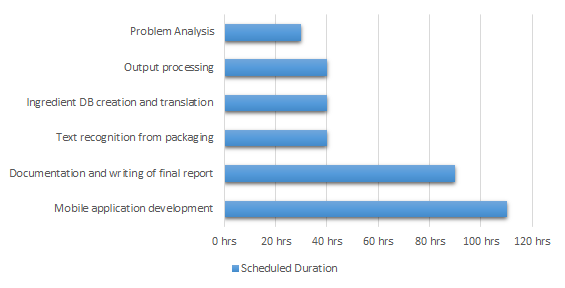
\includegraphics[width=\textwidth]{Figures/ganttbars.png}
  \caption{%
    Distribution of hours per development phase
  }
  \label{fig:ganttbars}
\end{figure}

This distribution was expected since the first tasks, without being any less relevant than the last, were focused on studying the literature and finding the right approach for the project. While some actual construction of the app was done at this steps, such as collecting and organizing the source data in a database or doing preliminary tests for the OCR implementation, most of the development was condensed on the last stages.